% This is the aspauthor.tex LaTeX file
% Copyright 2010, Astronomical Society of the Pacific Conference Series

\documentclass[11pt,twoside]{article}
\usepackage{asp2010}

\resetcounters


\markboth{Araya, Solar, Mardones, and Hochf\"arber}{Synthetic Data Cubes for Big
Data Algorithms}

\begin{document}

\title{Exorcising the Ghost in the Machine: Synthetic Spectral Data Cubes for
Assessing Big Data Algorithms}
\author{Mauricio~Araya$^1$, Mauricio~Solar$^1$, Diego Mardones$^2$ and Teodoro
Hochf\"arber$^1$}
\affil{$^1$Universidad T\'ecnica Federico Santa Mar\'ia, Avenida Espa\~na 1680, Valpara\'iso, Chile.}
\affil{$^2$Universidad de Chile, Camino El Observatorio 1515, Santiago, Chile.}

\begin{abstract}
The size and quantity of the data that is being generated by large astronomical
projects like ALMA, requires a paradigm change in astronomical data analysis.
Complex data, such as highly sensitive spectroscopic data in the form of large
data cubes, are not only difficult to manage, transfer and visualize, but they
also turn unfeasible the use of traditional data analysis techniques and
algorithms. Consequently, the attention have been placed on machine learning and
artificial intelligence techniques, to develop approximate and adaptive methods
for astronomical data analysis within a reasonable computational time.
Unfortunately, these techniques are usually sub optimal, stochastic and strongly
dependent of the parameters, which could easily turn into ``a ghost in the
machine'' for astronomers and practitioners. Therefore, a proper assessment of
these methods is not only desirable but mandatory for trusting them in
large-scale usage. The problem is that positively verifiable results are scarce
in astronomy, and moreover, science using bleeding-edge instrumentation
naturally lacks of reference values. We propose an Astronomical SYnthetic Data
Observations (ASYDO), a virtual service that generates synthetic spectroscopic
data in the form of data cubes. The objective of the tool is not to produce
accurate astrophysical simulations, but to generate a large number of labelled
synthetic data, to assess advanced computing algorithms for astronomy and to
develop novel Big Data algorithms. The synthetic data is generated using a set
of spectral lines, template functions for spatial and spectral distributions,
and simple models that produce reasonable synthetic observations. Emission lines
are obtained automatically using IVOA's SLAP protocol (or from a relational
database) and their spectral profiles correspond to distributions in the
exponential family. The spatial distributions correspond to simple functions
(e.g., 2D Gaussian), or to scalable template objects. The intensity, broadening
and radial velocity of each line is given by very simple and naive physical
models, yet ASYDO's generic implementation supports new user-made models, which
potentially allows adding more realistic simulations. The resulting data cube is
saved as a FITS file, also including all the tables and images used for
generating the cube. We expect to implement ASYDO as a virtual observatory
service in the near future.
\end{abstract}

\vspace{-0.5cm}

\section{Introduction}

The data deluge problem in astronomy is rapidly moving from a forecast to a
reality. Analyzing Astronomical Big Data (ABD) imposes new 
scientific challenges for astronomers that are not yet fully understood, meanwhile
massive astronomical datasets are starting to pile. There
is a growing consensus in the community that machine/statistical
learning and artificial intelligence techniques could be the key to cope with
ABD (\cite{ball2010data}), as they have been successfully applied in other Big Data domains. 
A common misconception when using these techniques is to think of them
as black-box machines, leading most of the times to mediocre results.
Therefore, a good integration of these techniques to astronomical data analysis
needs not only a proper understanding of the theory behind these methods, but
also a mechanism to assess the quality of the results.
%in order to perform a
%correct parameter selection and to tailor ad-hoc methods to the problem at hand.

%In particular, learning algorithms are highly data consuming in their raw state, 
%but this can be significantly lightened as we encode prior knowledge in our model. 
%On the other hand, including too strong priors can lead to a very poor learning rate.
%A similar dilemma is the algorithm's flexibility, where more general methods
%require to setup more free parameters. These and other similar issues can be
%overwhelming for an astronomer, in the sense that most of these parameters 
%are not in the astrophysical domain, but in the abstract space of the method
%parameters. Moreover, verifiable and labelled real 
%data is scarce in astronomy, which is a problem for applying supervised methods
%and for performing parameter sensitivity analysis. Another common problem is
%the curse of dimensionality, which means that techniques that works well
%in few dimensions or samples, do not generally scale up directly. Consequently,
%the use of heuristic and approximate methods, usually with a strong stochastic
%component, is a common practice in machine learning and artificial intelligence.
%All these problems, can easily generate the sense of a ``ghost in the machine'' 
%for practitioners, which can lead to discarding useful methods due to the lack
%of a proper test bench.

To tackle this issue, we propose generating synthetic astronomical data 
to test and evaluate 
complex algorithms and their parameters. The key idea is to use very simple
astrophysical models to generate a huge amount of data (ABD) that resembles 
real observations in terms of dimensionality, sparseness and complexity.

\section{Synthetic Spectroscopic Data Cubes}

The Atacama Large Millimeter/Submillimeter Array (ALMA) is currently generating
observations that clearly qualify as ABD, at least in the terms of
dimensionality and complexity. The main data products after correlation and
calibration are high resolution spectroscopic data cubes, which are not only
difficult to manage and visualize, but they also carry complex information about
the molecules of one or several sources, and their dynamics in the form of
emission lines \cite{teuben2013}.

A simple way to generate a synthetic cube is to use the following model for
a temperature of data cell:
\vspace{-0.5cm}
\begin{equation}
C(x,y,f)=\sum_{l \in \mathcal{L}(x,y,f)}
\int_{\nu_f - \Delta
\nu/2}^{\nu_f + \Delta \nu/2} 
Br(\nu,l)df + \epsilon,
\label{eq:base}
\end{equation}
where $x$ and $y$ are spatial indices and $f$ is a spectral index 
in the cube. For each line $l$ that emits in the field of view of that cell, 
there is a specific broadening function $Br()$ that sums accordingly to the spectral
resolution $\Delta \nu$ for that frequency. Also, an Gaussian noise $\epsilon$ is added 
to the model.

%For example, by assuming a simple Gaussian profile for all the lines, the model
%would be:
%\begin{equation}
%C(x,y,f)=\sum_{l \in \mathcal{L}(x,y,f,l)}
%\int_{\nu_f - \Delta
%\nu/2}^{\nu_f + \Delta \nu/2} 
%\frac{T_l(x,y)}{S_l(x,y) \sqrt{2\pi}}exp\left(- \frac{(\nu - \nu_l(1 +
%Z_l(x,y)))^2}{2S_l(x,y)^2}\right) df +
%\epsilon
%\label{eq:base}
%\end{equation}
%where $T_l$ is the intensity matrix, $S_l$ the broadening matrix
%(variance), and $Z_l$ the red-shift matrix of the line $l$. 
In practice, lines can be grouped by molecules and their
relative intensity can be randomly generated within reasonable
ranges obtained from the line's energy levels. 
Currently, the model used for generating these emission lines 
is a simplified version of the detection equation in \cite{stahler2008formation}.

\subsection{The ASYDO Package}

The Astronomical SYnthetic Data Observations tool (ASYDO), is
a python package that generates arbitrary spectroscopic data cubes
in the ALMA bands, based on mock astrophysical models.
ASYDO works under the Virtual Universe (VU) concept, which is
a persistent object that can hold several sources spread in a virtual
celestial sphere. Sources that belongs to this universe 
are defined by a central coordinate ($\alpha_S$, $\delta_S$) and a base
red-shift $z_S$. Each source can contain one or more components,
and each component uses one of the predefined astrophysical mock models (see
Figure~\ref{fig:models} (a)). 

\begin{figure}
\begin{minipage}{0.49\linewidth}
\centerline{(a)}
\centerline{\includegraphics[width=0.9\linewidth]{O1-5_f1.eps}}
\end{minipage}
%\begin{minipage}{0.3\linewidth}
%\centerline{(b)}
%\centerline{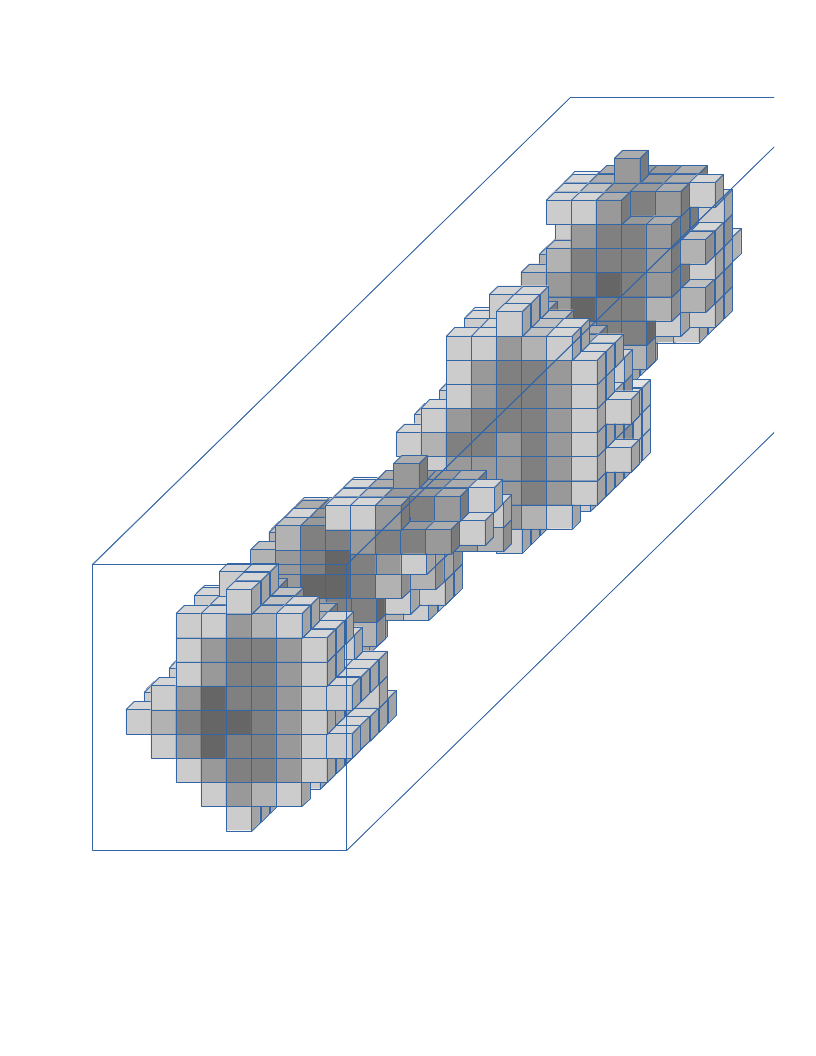
\includegraphics[width=0.9\linewidth]{cube-thresh3.png}}
%\end{minipage}
\begin{minipage}{0.49\linewidth}
\centerline{(b)}
\centerline{\includegraphics[width=0.7\linewidth]{O1-5_f2.eps}}
\end{minipage}
\caption{(a) Schematic of the virtual universe and the cube generation process.
(b) ASYDO main package components and their interactions, including the VU, DB
and Factory.}
\label{fig:models}
\end{figure}

After defining the sources of the universe, data cubes can be generated by
performing \emph{observations} to the virtual universe, by providing
the angular central position ($\alpha$,$\delta$), angular resolution
$\Delta\theta$ and the Field of View (FOV), as well as the
central frequency $\nu$, spectral resolution ($\Delta \nu$) and spectral
bandwidth (BW).

The main idea is that each model object knows how to project itself into a
specific data cube depending on its parameters and local definitions. This
allows, for example, generating cubes for the same region but with different
resolutions and/or bands.

\subsection{Tools for Building Models}

Even though ASYDO implements an example mock model for generating Interstellar
Molecular Clouds (IMC), the main idea of the package is to provide
the tools for developing custom models. Currently, ASYDO supports the
following functions:

\begin{itemize}
\item \textbf{Spatial structures}: 2D Gaussians, Generalized 2D Gaussians
(Saturated, Lorenzian) and Exponential
\item \textbf{Spectral distributions}: Gaussian and Skew-Normal
\item \textbf{Radial velocity gradients}: Linear and Exponential
\end{itemize}

The functions under development and testing are soft-edge rings and
random clouds for spatial structures, voigt profiles (with skew) for
spectral distributions, and noisy gradients for radial velocity.

Also, ASYDO provides an unified mechanism to querying spectral line
databases for models that require this information. A special module
in the package allows generating a SQLite database with a set of
spectral lines using IVOA's SLAP protocol, or directly from a CSV
file obtained from another database such as Splatalogue 
(see Figure~\ref{fig:models} (b)).

\subsection{FITS and the Cube Factory}

Each cube object contains also all the information used for
generating its temperatures. This cube can be exported
as a FITS file, that includes several images and tables:

\begin{itemize}
\item One 3D image that represents the actual cube
\item Three 2D images for each component, representing the temperature,
red-shift and broadening maps.
\item A binary table for each component, with each entry representing one line. 
The columns of the table are a unique line code, the molecule name, the
chemical name (formula), the rest frequency, the observed frequency, the base
red-shift, and optionally a reference temperature.
\end{itemize}

These cubes can be generated by defining each model parameters by hand, or
by using the \emph{cube factory} module. This module allows defining
ranges for the parameter values, from which each instance draws its parameters
uniformly. This module allows generating different cubes in parallel using all
the available cores for computing.

\subsection{A Simple Example}

We used the cube factory to generate 30000 data cubes of 25x25x1000 cells each, for a 2 GHz 
bandwidth around the 300 GHz spectrum. Each cube have sources with a random
radial velocity between 150 and 1000 km/s, a mean temperature ranging between 50
and 500 K and roughly 30\% of the visible molecules in the spectrum. Their fwhm,
skewness and radial velocity gradients also slightly vary from one cube to the
other. In the half of the cubes we have forced one molecule to be present
(Phosphapropynylidyne), and forced the other half to not have this molecule.
After training a Support Vector Machine (SVM) using the raw
data, we have tested the accuracy of classification, obtaining a pale 62\%. 
As the data is balanced, we can conclude that the
SVM is actually finding some patterns to detect the presence of
Phosphapropynylidyne. Please note that this accuracy can be significantly
improved with a more thoughtful application of SVM by using dimensionality
reduction and extracting relevant descriptors.

%Support Vector Machines (SVM) are a very popular supervised machine learning technique
%for classifying objects. A very naive approach is to simply apply an SVM to the
%raw data, without dimensionality reduction, kernel selection or extracting
%relevant statistical descriptors to simplify the problem. 
%\subsection{Line Identification}

%\begin{figure}
%\centerline{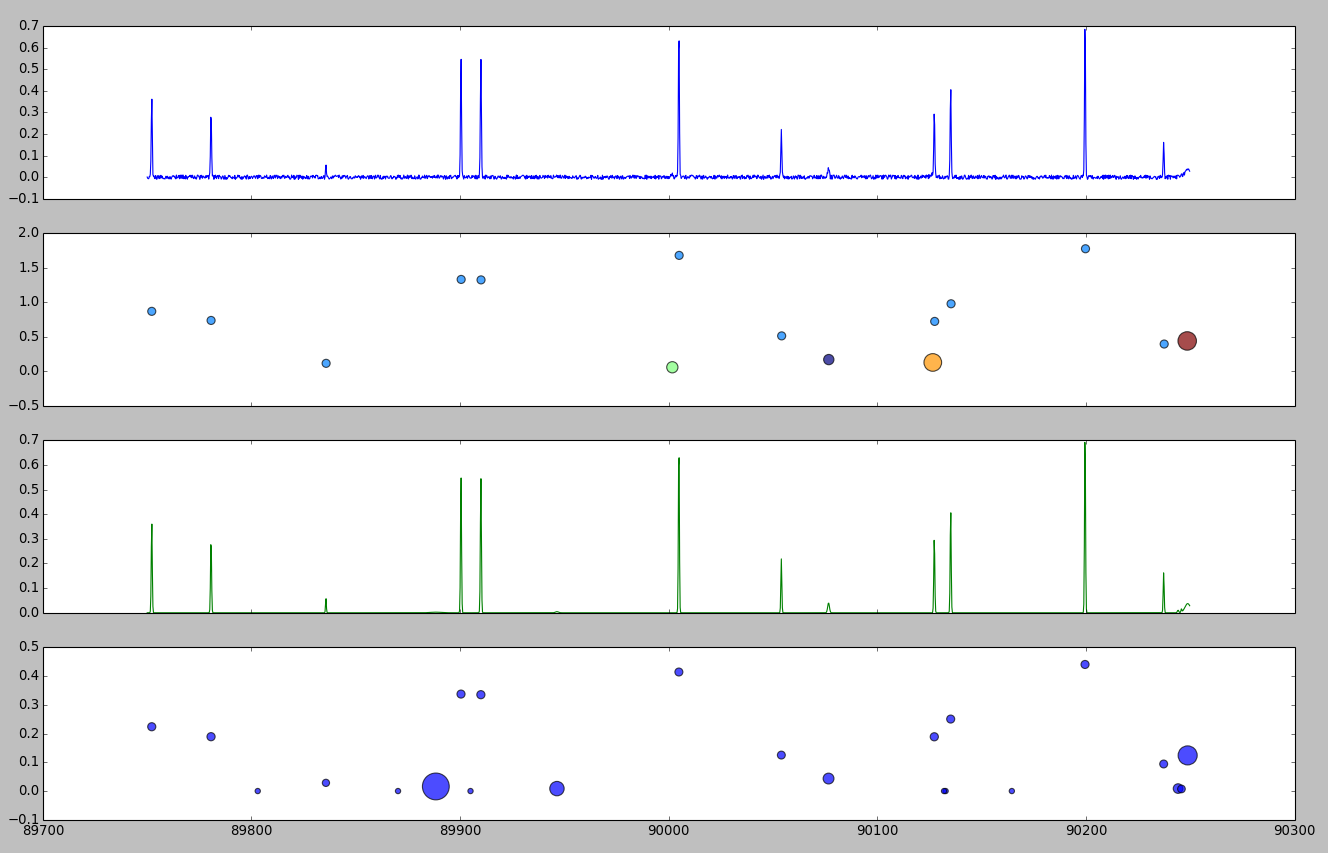
\includegraphics[width=0.95\linewidth]{good_fit.png}}
%\centerline{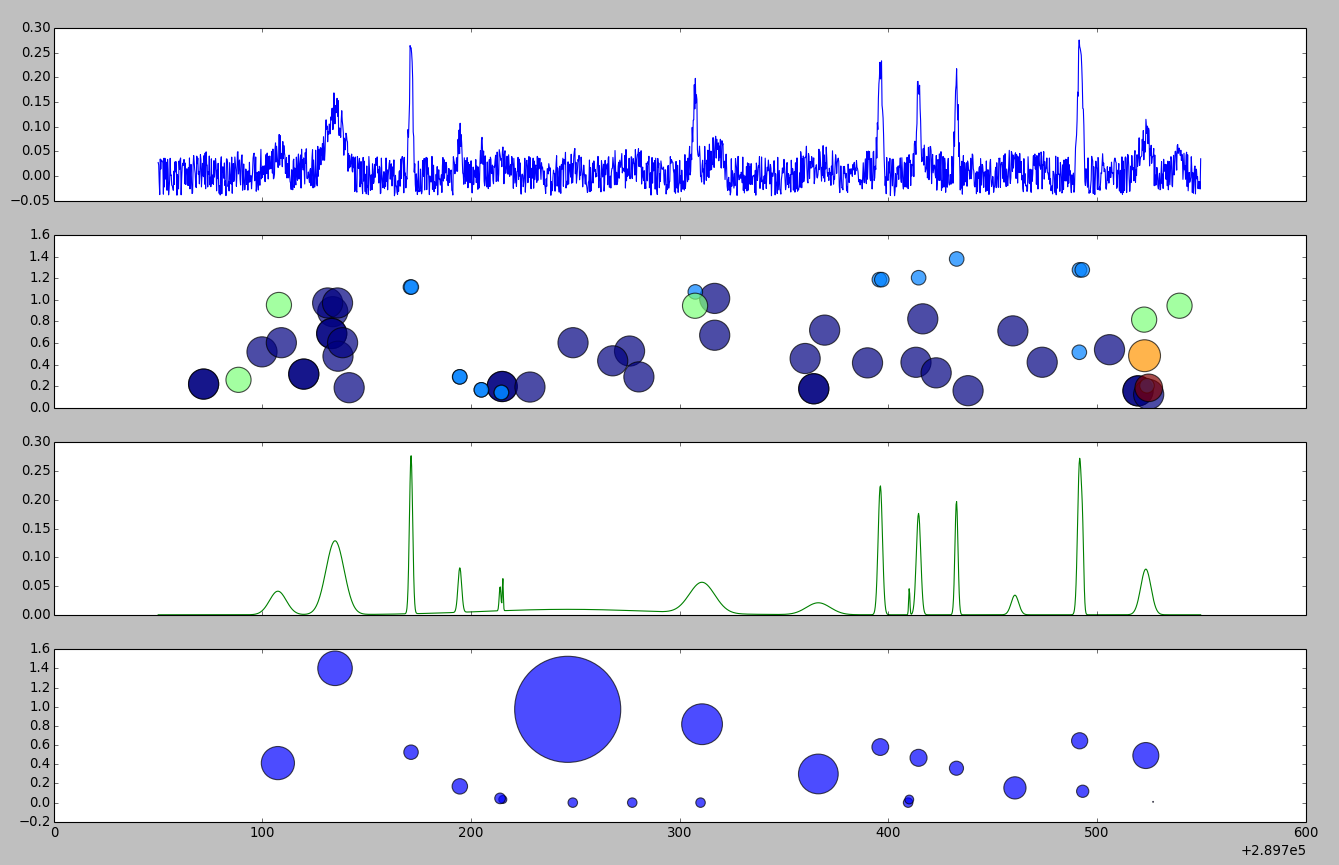
\includegraphics[width=0.95\linewidth]{toomany_fit.png}}
%\end{figure}

\section{Conclusions and Future Work}

We expect that ASYDO will help benchmarking machine learning
and artificial intelligence algorithms in order to produce
novel and ad-hoc methods for ABD. The SVM example shows that
synthetic data is useful for benchmarking algorithms, which
could lead to more adequate algorithms for the data at hand.
An interesting research direction is to train supervised 
algorithms using synthetic data to be used later with
real data, because gathering a large number of labelled data
is a complex task.

Besides increasing the variety of functions and models that 
ASYDO supports, we plan to improve the parallelization support
for high-performance computing environments. 
Also we expect to integrate this package as a
contributed package of astropy, and to develop an 
IVOA-like synthetic data generation standard to be
used a web-service.

%\section{The Template}
%To fill in this template, make sure that you read and follow the ASPCS Instructions for Authors and Editors available for download online.  Hints and tips for including graphics, tables, citations, and other formatting helps are available there.
%
%\subsection{The Author Checklist}
%The following checklist should be followed when writing a submission to a conference proceedings to be published by the ASP.
%
%\begin{itemize}
%\checklistitemize
%\item Article is within page limitations set by editor. 
%\item Paper compiles properly without errors or warnings.
%\item No fundamental modifications to the basic template are present, including special definitions, special macros, packages, \verb"\vspace" commands, font adjustments, etc. %(� 3.3, p. 10)
%\item Commented-out text has been removed. %(� 3.3, p. 10,11)
%\item Author and shortened title running heads are proper for the paper and shortened so page number is within the margin. %(� 3.1, p. 4)
%\item Paper checked for general questions of format and style, including, but not limited to, the following:
%\begin{itemize}
%  \item capitalization, layout, and length of running heads, titles  and \\sections/subsections;  % (� 3.1, p. 4) (� 3.2, p. 5) (� 3.3, p. 8)
%  \item page numbers within margin; % (� 3.1, p. 4)
%  \item author names spelled correctly and full postal addresses given; % (� 3.2, p. 5-6)
%  \item abstracts; % (� 3.2, p. 7);
%  \item all margins---left, right, top and bottom; % (�3.1, p. 4; �3.2, p. 5; �3.3, p. 9; �3.6, p. 21);
%  \item standard font size and no Type 3 fonts; %(� 3.3, pp. 10-11; � 3.6, p. 23; � 4.2, p. 25);
%  \item spacing; % (� 3.3, pp. 9-10);
%  \item section headings. % (� 3.3; p. 8).
%\end{itemize}
%\item All tables are correctly positioned within margins, are properly formatted, and are referred to in the text.  %(� 3.5, pp. 16-20)
%\item All figures are correctly positioned within margins, are minimum 300 dpi resolution, not too dark or too light, do not contain embedded fonts, and are referred to in the text.  All labeling or text will be legible with 10\% reduction.  Questionable images printed, checked and replaced if necessary.  Figures do not cover text or running heads, and proper permissions have been granted and acknowledged.  %(� 3.6, pp. 21-24)
%\item All acknowledgments and discussions are in proper format.  % (pp. 11-12, p. 20)
%\item If there are acknowledgments at the end of the article, ensure that the author has used
%the \verb"\acknowledgments" command and not the commands
%\\ \verb"\begin{Acknowledgments}", \verb"\end{Acknowledgments}".
%Acknowledgments should only be used for thanking institutions,
%groups, and individuals who have directly contributed to the work.
%\item All references quoted in the text are listed in the bibliography; all items in the bibliography have been referred to in the text.  % (� 4, pp. 24-28)
%\item All bibliography entries are in the proper format, using one of the referencing styles given. Each of the references is bibliographically complete, including full names of authors, editors, publishers, place of publication, page numbers, years, etc. % (�� 4.2-4.3, pp. 25-28)
%\item A complete Bib\TeX\ file is ready to submit to the editor.
%\item References to preprints replaced with publication information when possible.
%\end{itemize}

\acknowledgements{This research was funded by CONICYT through the FONDEF
D11I1060 and the ICHAA 79130008 projects.}

\bibliographystyle{asp2010}
\bibliography{O1-5}

\end{document}
